\providecommand{\main}{..}
\providecommand{\mintedoutdir}{\main/out/chapters}
\documentclass[\main/notes.tex]{subfiles}

\begin{document}
	\chapter{Graphics Systems and Models}
		\begin{definition}{Computer Graphics}
			All aspects of producing pictures or images using a computer.

			Began 50 years ago, with the display of lines on a \concept{cathode-ray tube (CRT)}.
		\end{definition}

		\begin{definition}{WebGL}
			A graphics software system supported by most modern web browsers.
			A version of \concept{OpenGL} -- the widely accepted standard for
			developing graphics applications.
		\end{definition}

		\section{Applications of Computer Graphics}
			\begin{sidenote}{Four Major Areas}
				\begin{center}
					\begin{enumerate*}[itemjoin=\quad]
						\item Display of information
						\item Design
						\item Simulation and animation
						\item User interface
					\end{enumerate*}
				\end{center}
			\end{sidenote}

			\subsection{Display of Information}
				\begin{example}[Types]
					\begin{itemize}[nosep]
						\item Floor plans
						\item Maps
						\item Statistics Plots
						\item Medical Imaging\\
							\begin{itemize*}[itemjoin=\quad]
								\item Computed Tomography (CT)
								\item Magnetic Resonance Imaging (MRI)
								\item Ultrasound
								\item Positron-emission tomography (PET)
							\end{itemize*}
						\item Scientific visualization
					\end{itemize}
				\end{example}
			\pagebreak

			\subsection{Design}
				Starting with a set of specifications, engines and architects seek a cost-effective
				and aesthetic solution that satisfies the specifications.
				Design is an iterative process.

				Design problems are either \concept{overdetermined} or \concept{underdetermined}.
				\begin{description}[nosep]
					\item[Overdetermined] No solution that satisfies all the criteria.
					\item[Underdetermined] Multiple solutions that satisfy all the criteria.
				\end{description}

				Using interactive graphic tools in \concept{computer-aided design (CAD)} occurs in many
				fields.

			\subsection{Simulation and Animation}
				An example is the training of pilots -- using graphical flight simulators increases safety,
				and reduces training expenses.

				The success of simulators led to using computer graphics for animation, as well as VR.

			\subsection{User Interfaces}
				The predominant way of interacting with computers uses a visual paradigm
				that includes windows, icons, menus, and a pointing device.

		\section{A Graphics System}
			\begin{sidenote}{Six Major Elements in a Graphics System}
				\vspace*{-0.5cm}
				\begin{multicols}{2}
					\begin{enumerate}[nosep]
						\item Input devices
						\item Central Processing Unit
						\item Graphics Processing Unit
						\item Memory
						\item Framebuffer
						\item Output devices
					\end{enumerate}
				\end{multicols}
			\end{sidenote}

			\subsection{Pixels and the Framebuffer}
				\begin{itemize}[nosep]
					\item Virtually all modern graphics systems are \concept{raster-based}.
					\item The image seen on the output device is an array -- the \concept{raster}
					-- of picture elements (\concept{pixels}), produced by the graphics system.
					\item Each pixel corresponds to a location in the image.
					\item The pixels are stored in a part of memory called the \concept{framebuffer}.
				\end{itemize}

				\begin{definition}{Framebuffer Properties}
					\begin{description}
						\item[Resolution] The number of pixels in the framebuffer.
						Determines the detail that can be seen in the image.
						\item[Depth (Precision)] The number of bits used for each pixel.
						Determines properties such as how many colors can be represented on a given system.
						For example, a 1-bit deep framebuffer would allow only two colors,
						whereas an 8-bit deep one would allow $2^8$ (256) colors.
					\end{description}
				\end{definition}

				\begin{sidenote}{Color Systems}
					\begin{description}
						\item[Full-color systems] 24 (or more) bits per pixel.
						These systems can display sufficient colors to represent most images realistically.
						These are also called \concept{true-color} systems, or \concept{RGB color} systems,
						because individual groups of bits in each pixel are assigned to each of the primary
						colors -- red, green, and blue -- that are used in most displays.
						\item[High dynamic range (HDR) systems] 12 or more bits for each color component
						(as opposed to the 8 above).
					\end{description}
				\end{sidenote}

				Until recently, framebuffers stored colors in integer formats.
				More recently, floating point has been used, which allows easier support for HDR.

				In a simple system, the framebuffer holds only the colored pixels displayed on the screen.
				However, in most systems, the framebuffer holds far more information, such as depth
				information.
				In these systems, the framebuffer contains multiple buffers, one of which is the
				\concept{color buffer}.

			\subsection{The CPU and GPU}
				In simple systems, there is a single processor, the \concept{central processing unit (CPU)},
				that performs both normal and graphical processing.
				The main graphical function of the processor is to take specifications of graphical
				primitives generated by application programs,
				and to assign values to the pixels in the framebuffer that best represent these entities.

				\begin{definition}{Rasterization}
					Also called \concept{scan conversion}.
					The conversion of geometric entities to pixel colors and locations in the framebuffer.

					\begin{example}[Triangle Rasterization]
						A triangle is specified by three vertices,
						but to display its outline by the three line segments connecting the vertices,
						the graphics system must generate a set of pixels that appear as line segments to the
						viewer.
					\end{example}
				\end{definition}

				In early graphics systems, the framebuffer was part of the standard memory
				that could be directly addressed by the CPU.

				Nowadays, virtually all graphics systems are characterized by special purpose
				\concept{graphics processing units (GPUs)} that are custom-tailored
				to carry out specific graphics functions.
				The GPU can be located on the motherboard, or on a graphics card.
				The framebuffer is accessed through the GPU and is usually on the same circuit board
				as the GPU.
			\pagebreak

			\subsection{Output Devices}
				\begin{wrapfigure}{r}{0.5\textwidth}
					\begin{center}
						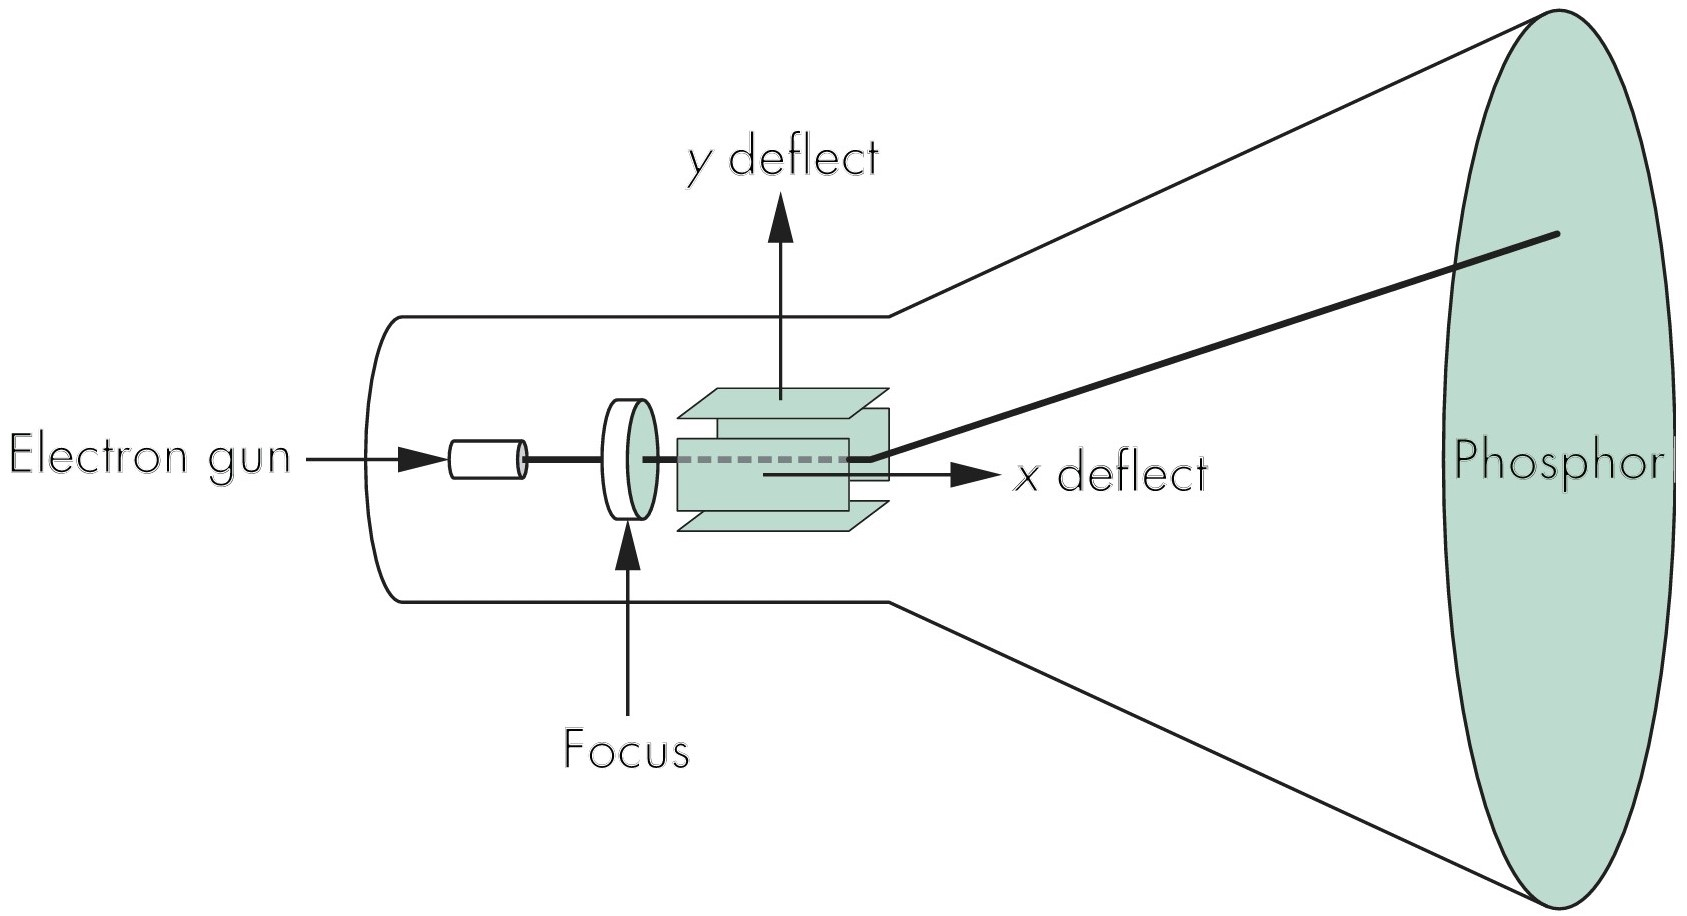
\includegraphics[width=0.48\textwidth]{\main/images/chapter01/cathode_ray_tube.jpg}
					\end{center}
					\caption{Cathode-Ray Tube (CRT)}
				\end{wrapfigure}

				Until recently, the dominant type of display (or \concept{monitor}) was the
				\concept{cathode-ray tube (CRT)}.

				When electrons strike the phosphor coating on the tube, light is emitted.
				The direction of the beam is controlled by two pairs of deflection plates.

				The output of the computer is converted, by digital-to-analog converters,
				to voltages across the $x$ and $y$ deflection plates.
				Light appears on the surface of the CRT when a sufficiently intense beam of electrons
				is directed at the phosphor.

				A typical CRT emits light for a short time -- usually a few milliseconds
				-- after the phosphor is excited by the electron beam.
				For a human to see a steady, flicker-free image, the same path must be \concept{refreshed},
				by the beam at a sufficiently high rate, called the \concept{refresh rate}.
				In older systems, the refresh rate was determined by the frequency of the power system:
				60 Hz in the US, and 50 Hz in much of the rest of the world.

				\begin{definition}{Vector CRT}
					If the voltages steering the beam change at a constant rate,
					the beam will trace a straight line, visible to the viewer.
					This is called the \mbox{\concept{random-scan}}, \concept{calligraphic},
					or \concept{vector} CRT,
					because the beam can be moved directly from any position to any other position.
					This is the basis of early graphics systems that predated the present raster technology.
				\end{definition}

				\begin{definition}{Raster CRT}
					In a raster system, the graphics system takes pixels from the framebuffer and
					displays them as points on the surface of the display in one of two ways:
					\begin{descriptimize}[nosep]
						\item[Noninterlaced] Pixels are displayed row by row,
						or scan line by scan line, at the refresh rate.
						\item[Interlaced] Odd rows and even rows are refreshed alternately.
						Used in commercial television.
						If the display is operating at 60 Hz, the screen is redrawn only 30 times per second.
					\end{descriptimize}
				\end{definition}

				Color CRTs have three different-colored phosphors (red, green, and blue),
				arranged in small groups.
				A common style is to arrange them in triangular groups called \concept{triads},
				where each triad consists of three phosphors: one for each primary color.
				Most color CRTs have three electron beams, corresponding to the types of phosphors.

				In the shadow-mask CRT, a metal screen with small holes (the \concept{shadow-mask})
				ensures that an electron beam excites only phosphors of the proper color.

				CRTs are still common display devices, but are being replaced by flat-screen technologies.
				Flat-panel monitors are inherently raster-based.
				All technologies available -- including light-emitting diodes (LEDs),
				liquid-crystal displays (LCD's), and plasma panels --
				use a two-dimensional grid to address individual light-emitting elements.
				\pagebreak

				\begin{wrapfigure}{l}{0.5\textwidth}
					\begin{center}
						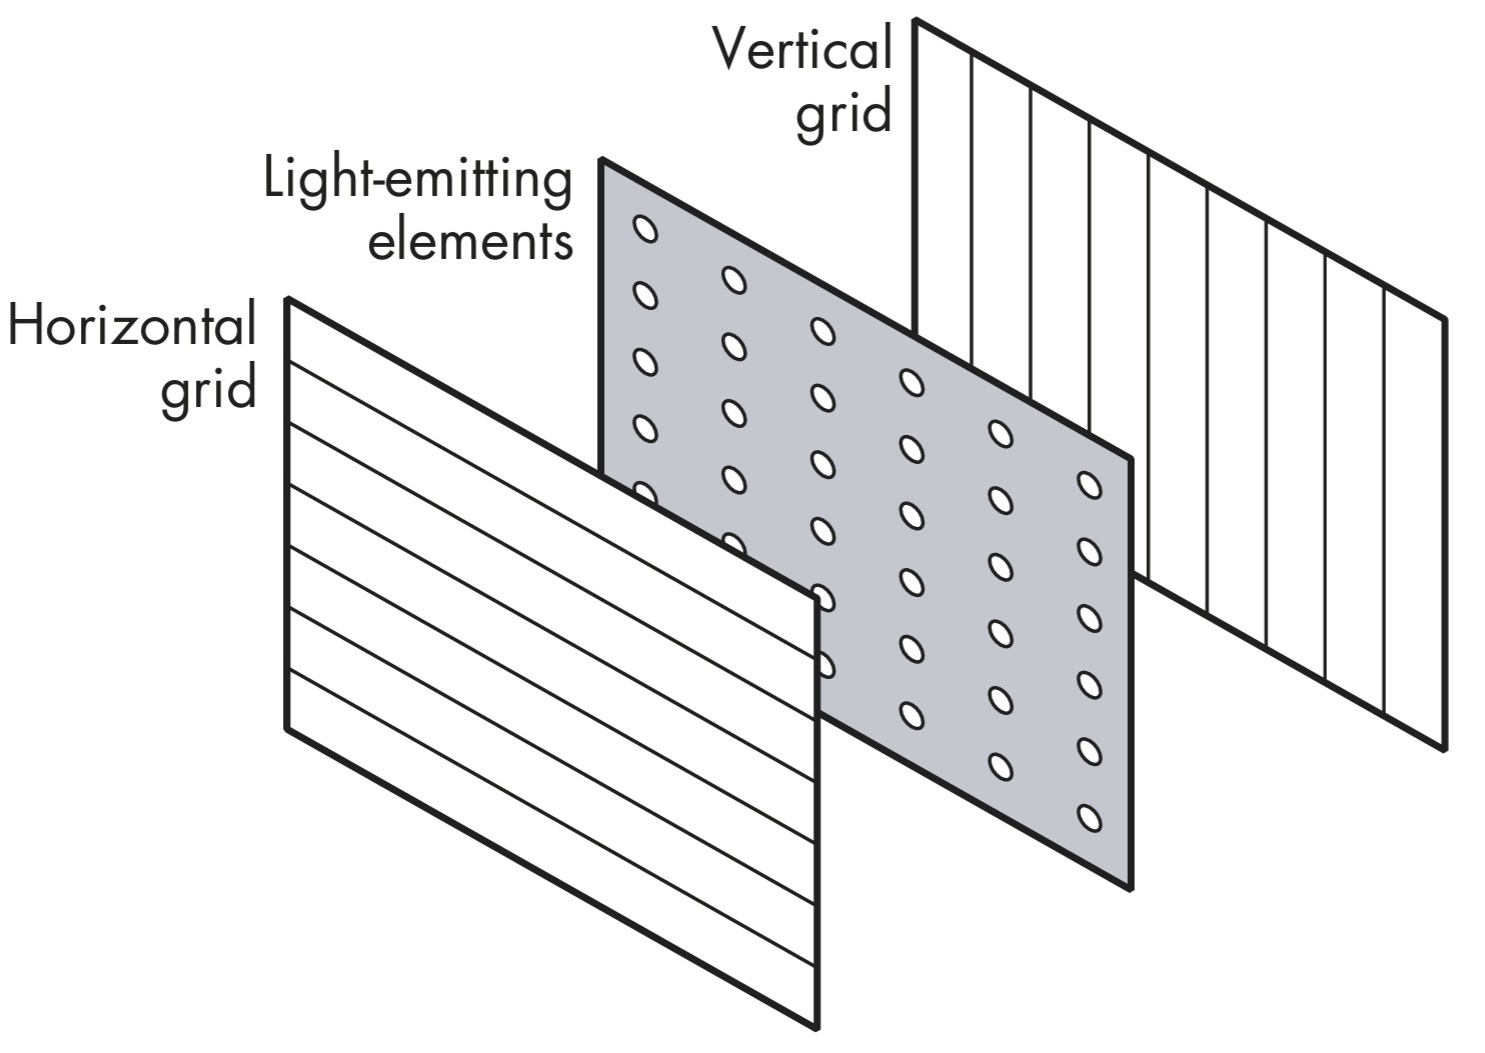
\includegraphics[width=0.48\textwidth]{\main/images/chapter01/flat_panel_display.jpg}
					\end{center}
					\caption{Generic Flat-Panel Display}
				\end{wrapfigure}

				A flat-panel display works as follows:

				The two outside plates each contain parallel grids of wires that are oriented perpendicular
				to each other.
				By sending electrical signals to the proper wire in each grid,
				the electrical field at the intersection of the two wires
				can be made strong enough to control the corresponding element in the middle plate.

				The middle plate in an LED panel contains light-emitting diodes
				that can be turned on and off by the electrical signals sent on the grid.
				In an LCD, the electrical field controls the polarization of the liquid crystals in
				the middle panel,
				thus turning on and off light passing through the panel.
				A plasma panel uses the voltages on the grids to energize gases embedded between the
				glass panels holding the grids.
				The energized gas becomes a glowing plasma.

				Most projection systems are raster-based.
				They use a variety of technologies including CRTs and digital light projection (DLP).
				These systems act as standard monitors with similar resolutions and perspectives.
				Hard-copy devices, such as printers and plotters, are also raster-based, but cannot be
				refreshed.

				Stereo (3D) television displays use alternate refresh cycles to switch the display
				between an image for the left eye and an image for the right eye.
				The viewer wears special glasses that are coupled to the refresh cycle.

			\subsection{Input Devices}
				Most graphics systems provide a keyboard and at least one other input device.
				The most common input devices are the mouse, the joystick, and the data tablet.
				Each of these provides positional information to the system,
				and is usually equipped with one or more buttons to provide signals to the processor.
				These devices are often called \concept{pointing devices},
				and allow a user to indicate a particular location on the display.

				Due to new input devices appearing regularly,
				our graphics programs should implement a flexible model for incorporating input devices.
			\pagebreak

		\section{Images: Physical and Synthetic}
			\subsection{Objects and Viewers}
				Every image formation process contains two basic entities:
				\concept{object} and \concept{viewer}.
				The object exists in space independent of any image formation process, and any viewer.
				In computer graphics, objects are formed by specifying positions in space of various
				geometric primitives.
				A set of locations in space, or of \concept{vertices}, is sufficient to define or
				approximate most objects.

				To form an image from an object, we need someone or something that is viewing the object.
				The \emph{viewer} forms the image of our objects.
				In the human visual system, the image is formed on the back of the eye.
				In a camera, the image is formed in the film plane.
				An image is a specific \emph{view} of an object -- viewers in a different relative
				location will have different images of the same object.

				Objects and viewers exist in three-dimensional space,
				but the image that is defined is two-dimensional.

			\subsection{Light and Images}
				An image must have a light source.
				Light from the source strikes various surfaces of the object,
				and a portion of the reflected light enters the camera through the lens.

				\begin{definition}{Light}
					A form of magnetic radiation.

					Electromagnetic energy travels as waves that can be characterized either by
					their wavelengths or their frequencies.
					The electromagnetic spectrum includes radio waves, infrared, and a portion that
					causes a response in our visual systems.

					This \concept{visual spectrum} is called \concept{light},
					and has wavelengths in the range of $350$ to $780$ nanometers (nm).

					A given light source has a color determined by the energy that it emits at various
					wavelengths.

					\begin{indentparagraph}
						\begin{descriptimize}[nosep]
							\item[450 nm] blue
							\item[520 nm] green
							\item[650 nm] red
						\end{descriptimize}
					\end{indentparagraph}
				\end{definition}

				Light sources can emit light either as a set of discrete frequencies,
				or over a continuous range.

				In computer graphics, we rarely need to deal with the physical properties of light.
				Instead, we use \concept{geometric optics}.

				\begin{definition}{Geometric Optics}
					This method models light sources as emitters of light energy,
					each of which have a fixed intensity.

					In this model, light travels in straight lines,
					from the sources to those objects with which it interacts.
				\end{definition}

				An ideal \concept{point source} emits energy from a single location
				at one or more frequencies equally in all directions.
				A particular source is characterized by the
				intensity of light it emits at each frequency and
				by that light's directionality.

			\subsection{Imaging Models}
				There are multiple approaches to forming images from a set of objects,
				the light-reflecting properties of these objects, and
				the properties of the light sources in the scene.

				We can start by building an imaging model by following light from a source.

				\begin{definition}{Ray}
					A semi-infinite line that emanates from a point and
					travels to infinity in a particular direction.
				\end{definition}

				Because light travels in straight lines, we can think in terms of rays of light
				emanating in all directions from our point source.
				A portion of these infinite rays contributes to the image on the film plane of our camera.
				Most of the rays go off to infinity, neither entering the camera directly nor striking any
				of the objects.
				The remaining rays strike and illuminate objects.

				\concept{Ray tracing} and \concept{photon mapping} are image formation techniques
				that are based on these ideas and that can form the basis for producing computer-generated
				images.
				We can use ray-tracing to simulate complex physical effects,
				if we are willing to carry our the requisite computing.
				Ray-tracing is usually not well-suited for real-time computation.

				Other physical approaches to image formation are based on conservation of energy.
				The most important in computer graphics is \concept{radiosity},
				which works best for services that scatter the incoming light equally in all directions.
				However, radiosity still requires more computation than can be done in real time.

		\section{Imaging Systems}
			\subsection{Pinhole Camera}
				\begin{definition}{Pinhole Camera}
					A box with a small hold in the center of one side:
					the film is placed inside the box on the side opposite the pinhole.
				\end{definition}
				\begin{example}[Pinhole Camera]
					\begin{wrapfigure}[7]{r}{0.5\textwidth}
						\begin{center}
							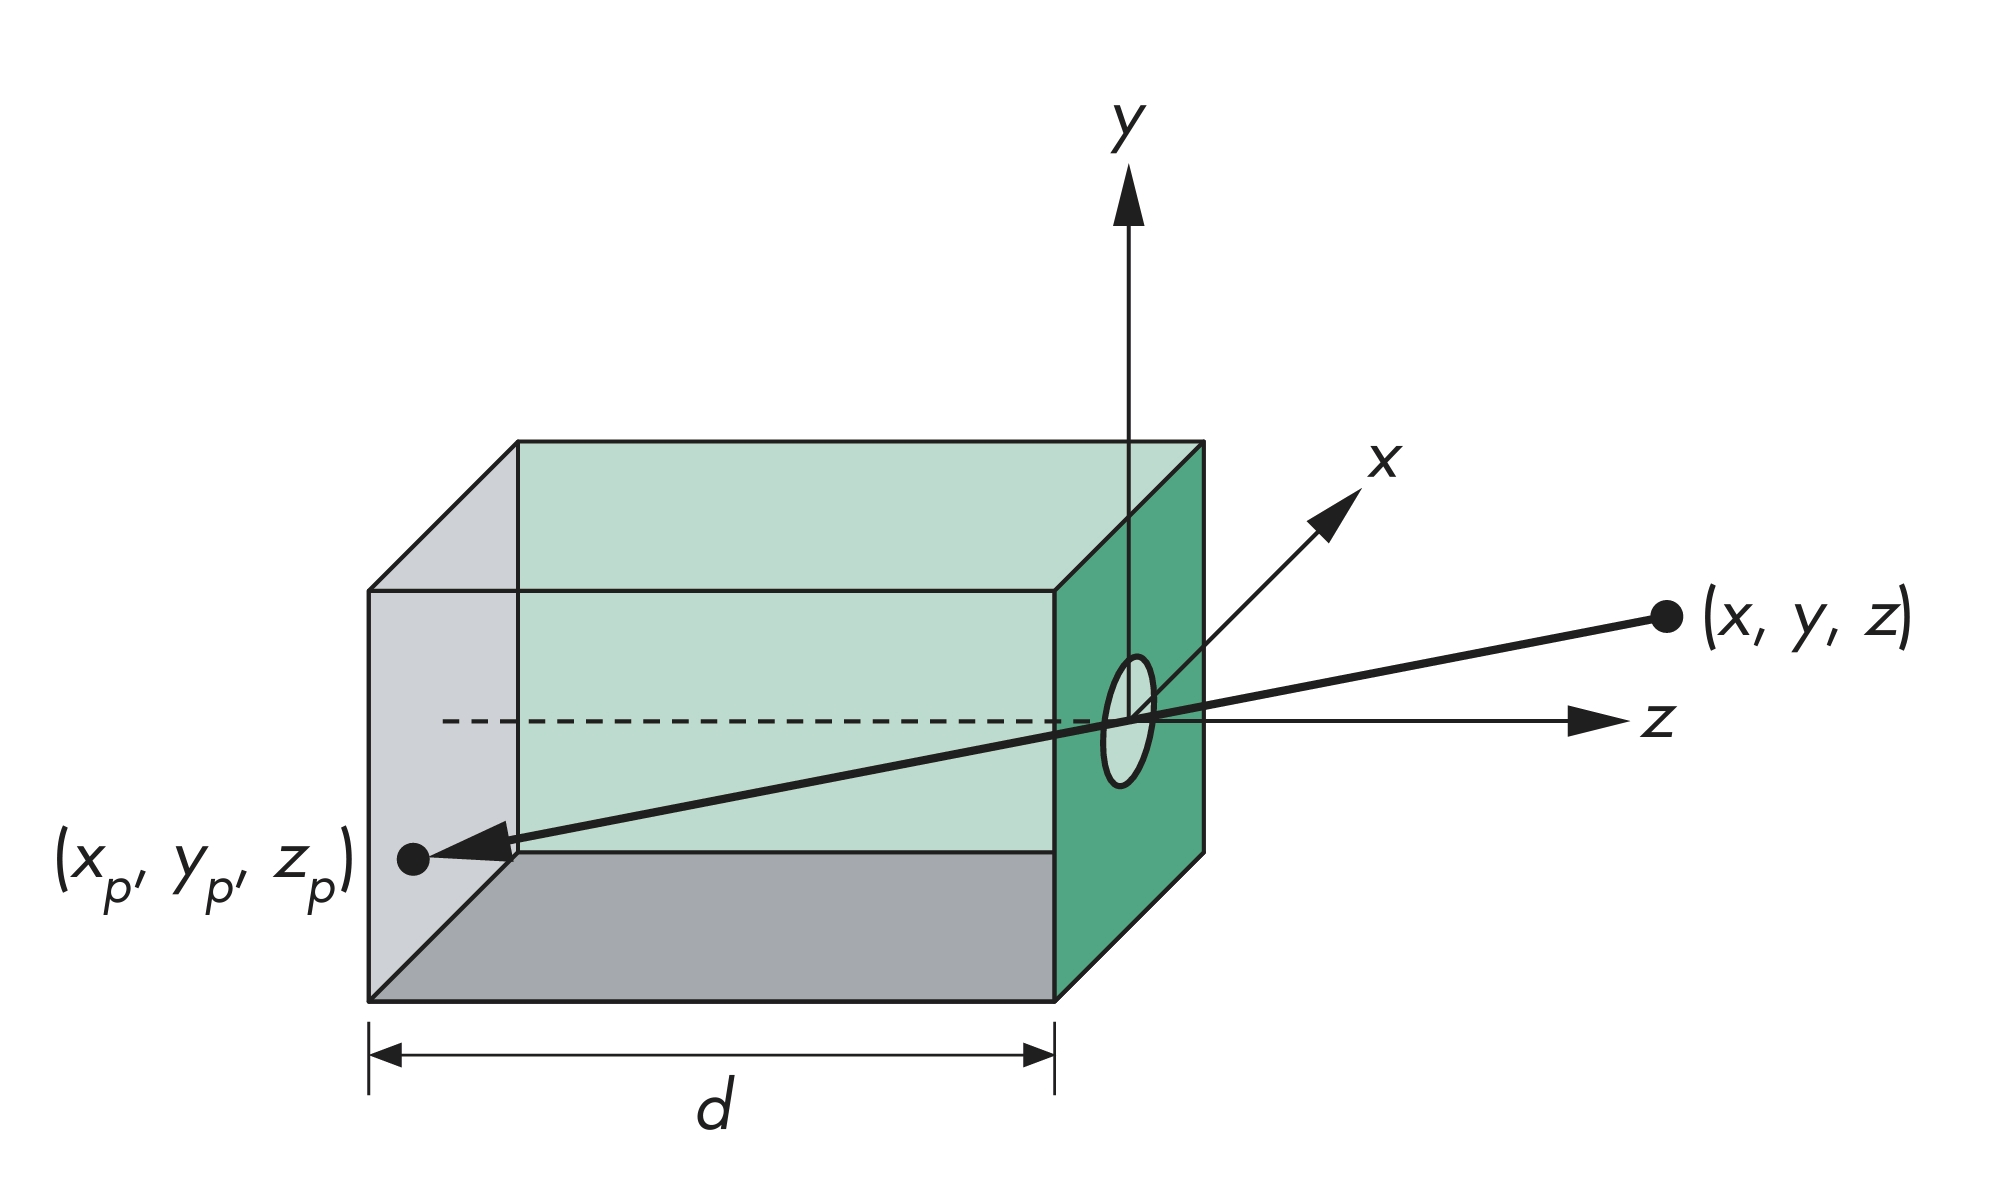
\includegraphics[width=0.48\textwidth]{\main/images/chapter01/pinhole_camera.png}
						\end{center}
						\caption{Pinhole Camera}
					\end{wrapfigure}

					Suppose the camera is oriented along the \mbox{$x$-axis},
					with the pinhole at the origin of our coordinate system.

					Assume the hole is so small that only a single ray of light,
					emanating from a point, can enter it.
					The film plane is located at a distance $d$ from the pinhole.

					\vspace{4.5em}
					\pagebreak

					\begin{wrapfigure}[11]{l}{0.5\textwidth}
						\vspace{-20pt}
						\begin{center}
							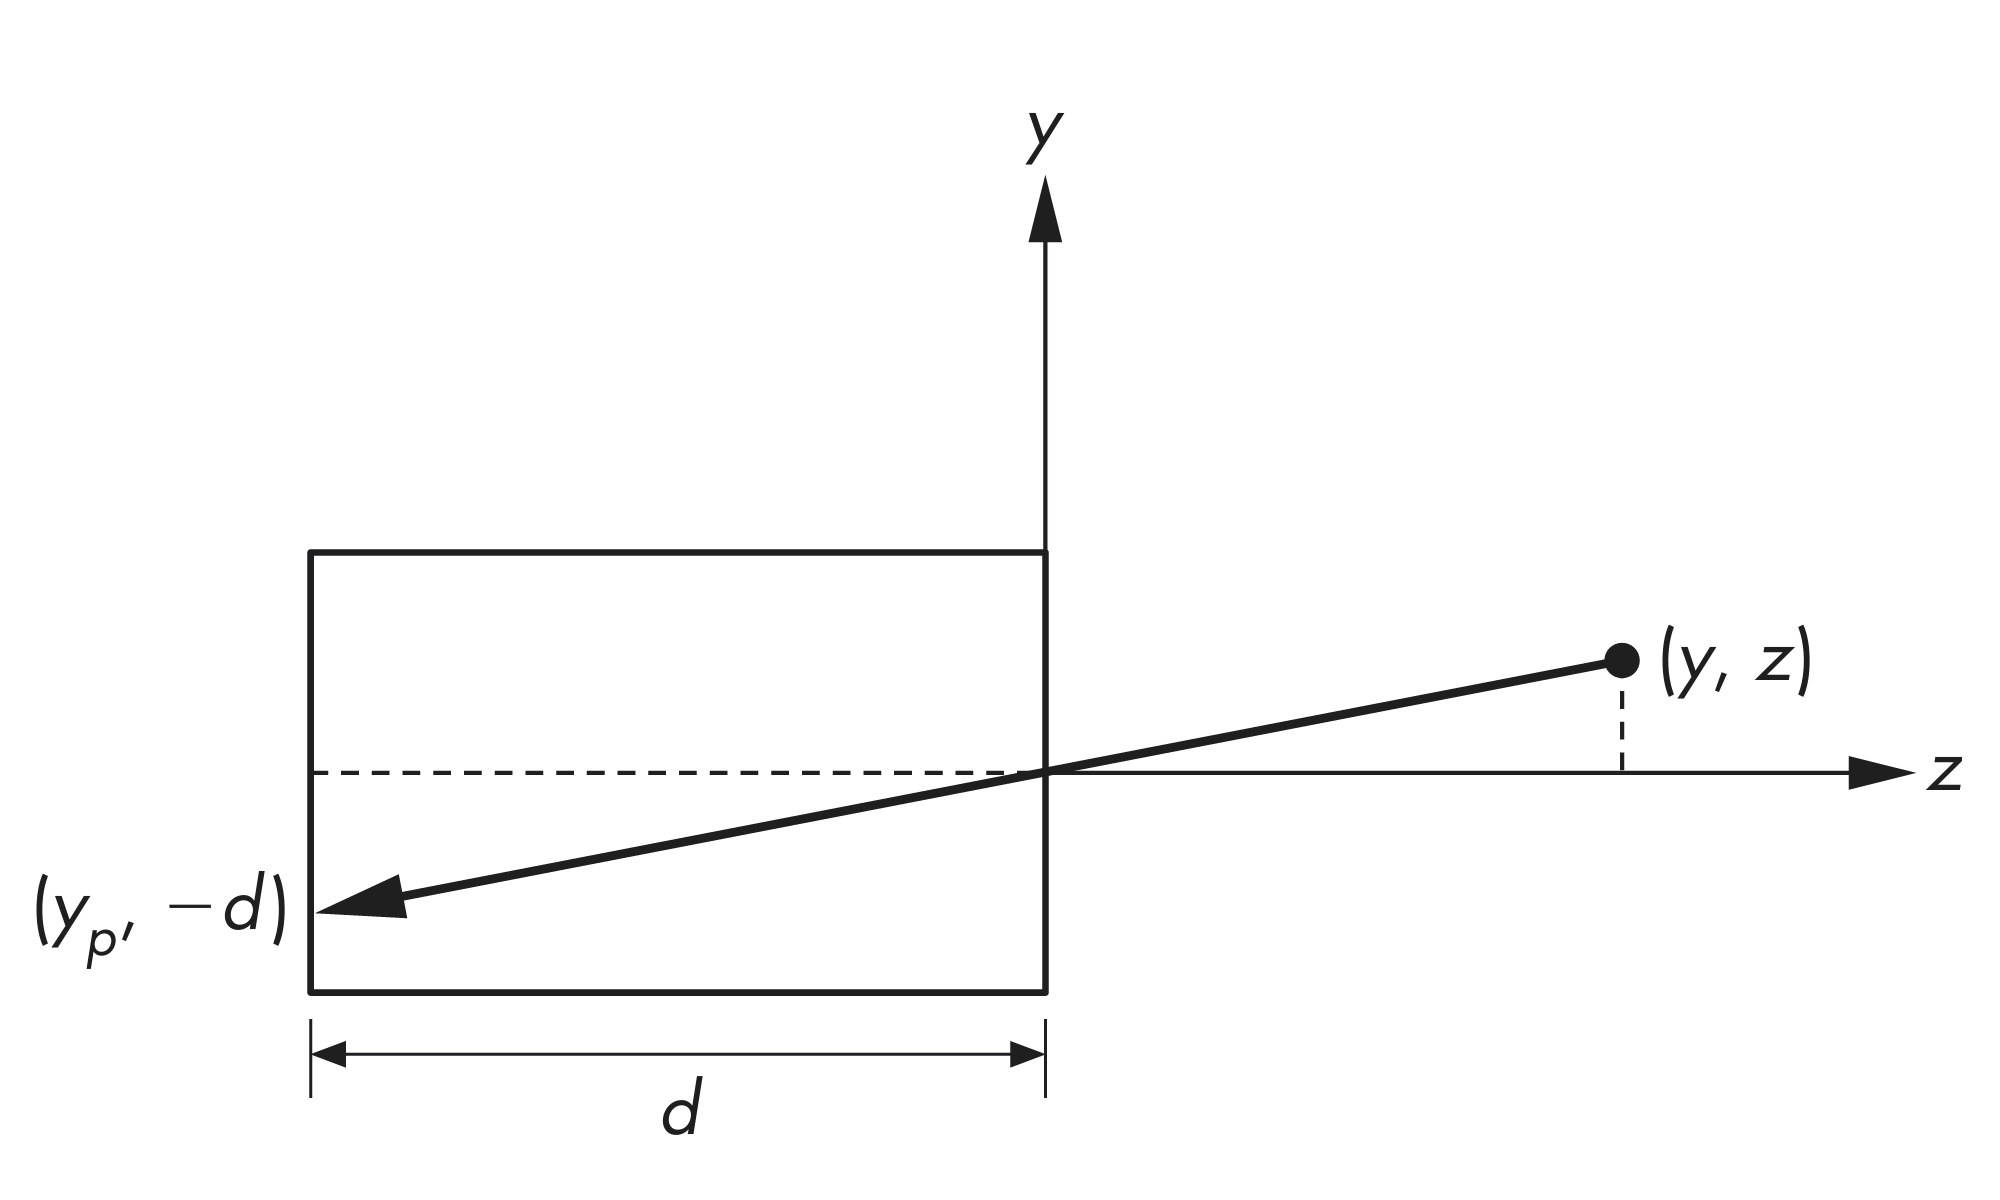
\includegraphics[width=0.48\textwidth]{\main/images/chapter01/pinhole_camera_side.png}
						\end{center}
						\vspace{-10pt}
						\caption{Pinhole Camera Side View}
					\end{wrapfigure}

					A side view allows us to calculate where the image of the point ($x$, $y$, $z$) is
					on the film~plane~$z = -d$.
					As the two triangles are similar, the $y$ coordinate of the image is at $y_p$.
					\begin{align*}
						y_p &= -\frac{y}{z/d}
					\end{align*}

					Using a top view, a similar calculation is:
					\begin{align*}
						x_p &= -\frac{x}{z/d}
					\end{align*}

					The point ($x_p$, $y_p$, $-d$) is called the \concept{projection}
					of the point ($x$, $y$, $z$).
					The color on the film plane at this point will be the color of the point ($x$, $y$, $z$).
				\end{example}

				The \concept{field of view} (or \concept{angle of view}) is
				the angle made by the largest object that our camera can image on its film plane.
				If $h$ is the height of the camera, the angle of view $\theta$ is:
				\begin{align*}
					\theta &= 2\tan^{-1}\left(\frac{h}{2d}\right)
				\end{align*}

				The ideal pinhole camera has an infinite \concept{depth of field}:
				every point within its view is in focus.
				Every point in its field of view projects to a point on the back of the camera.

				The pinhole camera has two disadvantages:
				the pinhole is small, so almost no light enters the camera; and
				the camera cannot be adjusted to have a different field of view.

				To resolve the above issues, the pinhole can be replaced with a lens.
				Firstly, the lens gathers more light than can pass through the pinhole:
				the larger the aperture of the lens, the more light the lens can collect.
				Secondly, by picking a lens with the proper focal length
				(equivalent to choosing the distance $d$ for the pinhole camera)
				we can achieve any desired field of view (up to 180 degrees).
				Lenses, however, do not have an infinite depth of field:
				not all distances from the lens are in focus.

				Like the pinhole camera, computer graphics produces images in which
				all objects are in focus.

			\subsection{The Human Visual System}
				Light enters the eye through the cornea (a transparent structure that protects the eye),
				and the lens.
				The iris opens and closes to adjust the amount of light entering the eye.
				The lens forms an image on a two-dimensional structure called the \concept{retina}
				on the back of the eye.
				The rods and cones are light sensors and are located on the retina.
				They are excited by electromagnetic energy in the range of 350 to 780 nm.

				The rods are low-level-light sensors that account for our night vision,
				and are not color-sensitive;
				the cones are responsible for our color vision.
				The sizes of the rods and cones, and the optical properties of the lens and cornea,
				determine our \concept{visual acuity} or the \concept{resolution} of our visual systems.

				\begin{definition}{Resolution (of the eye)}
					A measure of what size objects we can see.
					That is, a measure of how close we can place two points
					and still recognize that there are two distinct points.
				\end{definition}

				The sensors in the human eye react differently to light energy at different wavelengths.
				There are three types of cones and a single type of rod.
				Intensity and brightness are different:
				one is a physical measure, the other is a measure of perception.

				\begin{definition}{Brightness}
					A measure of how intense we perceive the light emitted from an object to be.

					An overall measure of how we react to the intensity of light.
				\end{definition}

				The human visual system reacts differently to monochromatic green light than to red.
				If these lights emitted the same energy, they would appear to have different brightness.
				The human eye is most sensitive to green light, and least sensitive to red and blue.

				As there are three different cone types,
				instead of working with all visible wavelengths individually,
				we can use three standard primaries to approximate any color that we can perceive.

		\section{The Synthetic-Camera Model}
			\begin{definition}{Synthetic-Camera Model}
				Look at creating a computer-generated image as being similar to
				forming an image using an optical system.
			\end{definition}

			\begin{sidenote}{Principles for the Synthetic-Camera Model}
				\begin{enumerate}[nosep]
					\item The specification of objects is independent of the specification of the viewer.
					\item We can compute an image using simple geometric calculations.
				\end{enumerate}
			\end{sidenote}

			With a real camera, the image of the object is flipped relative to the object.
			The film needs to flipped to regain the original orientation of the object.

			For a synthetic camera, the above can be avoided by
			drawing another plane in front of the lens, and
			working in three dimensions.
			We find the image of a point on the object on the virtual plane
			by drawing a line, called a \concept{projector}
			from the center of the lens (called the \concept{center of projection (COP)}).
			All projectors are rays emanating from the center of projection.
			In a synthetic camera, the virtual image plane that is moved in front of the lens
			is called the \concept{projection plane}.

			The size of an image is limited.
			In the pinhole camera, the field of view expresses this limitation.
			In the synthetic camera, this limitation can be moved to the front by
			placing a \concept{clipping rectangle} or \concept{clipping window}
			in the projection plane.
			This rectangle acts as a window through which a viewer,
			located at the center of projection,
			sees the world.
			Given the location of the center of projection,
			the location and orientation of the projection plane, and
			the size of the clipping rectangle,
			we can determine which objects will appear in the image.

		\pagebreak

		\section{The Programmer's Interface}
			\begin{definition}{Application Programming Interface (API)}
				A set of functions in a graphics library that defines the interface
				between an application program and a graphics system.
			\end{definition}

			The application programmer sees only the API,
			and is not concerned with the details of both the hardware and software implementation
			of the graphics library.

			\begin{definition}{Software Drivers}
				Responsible for interpreting the output of the API
				and converting these data to a form that is understood by the particular hardware.
			\end{definition}

			The functions of the API should match the conceptual model
			that the user wishes to employ to specify images.

			\subsection{The Pen-Plotter Model}
				Most early graphics systems were two-dimensional.
				The model they used is referred to as the \mbox{\concept{pen-plotter model}},
				due to the output device that was available on these systems.

				\begin{definition}{Pen Plotter}
					A device that produces images by moving a pen held by a \concept{gantry},
					a structure that can move the pen in two orthogonal directions across the paper.

					The plotter can raise and lower the pen as required to create the desired image.

					They view the process of creating an image as being similar to the process of
					drawing on a pad of paper.
				\end{definition}

				\begin{example}[Pen-Plotter Functions]
					\begin{minted}[autogobble, bgcolor={example color!25!white}]{javascript}
						moveto(x, y);
						lineto(x, y);
					\end{minted}
					\mintinline{javascript}|moveto(x, y)| moves the pen to the location ($x$, $y$)
					on the paper without leaving a mark.
					\mintinline{javascript}|lineto(x, y)| moves the pen to the location ($x$, $y$)
					on the paper while drawing a line from the old location to the new location.
				\end{example}

				A different raster-based (but still limited) two-dimensional model
				relies on writing pixels directly into a framebuffer.
				This could use the function:
				\begin{minted}[autogobble]{javascript}
					writePixel(x, y, color);
				\end{minted}
				where \mintinline{javascript}|x, y| is the location of the pixel in the framebuffer
				and \mintinline{javascript}|color| is the color to be written there.

				The pen-plotter method does not extend well to three-dimensional graphics systems.

			\subsection{Three-Dimensional APIs}
				The synthetic-camera model is the basis for a number of popular APIs.
				This requires functions to specify the following:
				\begin{center}
					\begin{itemize*}[itemjoin=\quad]
						\item objects
						\item a viewer
						\item light sources
						\item material properties
					\end{itemize*}
				\end{center}

				\subsubsection{Objects}
					Objects are usually defined by a set of \concept{vertices}.
					For simple geometric objects, there is a simple relationship between a list of vertices
					(positions in space)
					and the object.
					For more complex objects, there may be multiple ways of defining the object
					from a set of vertices.

					\begin{example}[Circle]
						A circle can be defined by three points on its circumference,
						or by its center and one point on its circumference.
					\end{example}

					Most APIs provide similar sets of primitive objects for the user
					-- usually those that can be displayed rapidly on the hardware.
					These include points, line segments, and triangles.

					WebGL programs specify primitives through a set of vertices.

					\begin{example}[Defining Vertices in Javascript]
						\begin{minted}[autogobble, bgcolor={example color!25!white}]{javascript}
							var vertices = [ ];

							vertices[0] = [0.0, 0.0, 0.0]; // Vertex A
							vertices[1] = [0.0, 1.0, 0.0]; // Vertex B
							vertices[2] = [0.0, 0.0, 1.0]; // Vertex C
						\end{minted}

						These vertices only give three locations in a three-dimensional space
						-- they do not specify the geometric entity that they define.

						The choice of what entity is being defined is specified by
						setting a parameter corresponding to the geometric entity we would like these locations
						to specify.

						Regardless of the geometric entity, we specify the geometry
						and let the graphics system determine which pixels to color in the framebuffer.
					\end{example}

					Some APIs let the user work directly in the framebuffer by
					providing functions that read and write pixels.
					Additionally, some APIs provide curves and surfaces as primitives.
					WebGL provides access to the framebuffer through texture maps.

				\pagebreak

				\subsubsection{Viewer}
					There are a variety of ways to define a viewer or camera.
					There are four necessary specifications:
					\begin{indentparagraph}
						\begin{descriptenum}[nosep]
							\item[Position] The camera location is usually given by the position of 
								the center of the lens, which is the center of projection (COP).
							\item[Orientation] Once the camera is positioned,
								we can place a camera coordinate system
								with its origin at the center of projection.
								The camera can then be rotated independently around the three axes of the system.
							\item[Focal length] Determines the size of the image on the film plane,
								that is, the portion of the world the camera sees.
							\item[Film plane] The back of the camera has a height and a width.
								On the bellows camera, and in some APIs, the orientation of the back of the camera
								can be adjusted independently to the orientation of the lens.
						\end{descriptenum}
					\end{indentparagraph}

					There are different ways to specify these specifications.
					One way to develop the specifications for the camera location and orientation
					is through a series of coordinate-system transformations.
					These transformations convert object positions
					represented in a coordinate system that specifies object vertices
					to object positions in a coordinate system centered at the COP.

					Having many parameters to adjust can make it difficult to get a desired image.
					Part of the problem lies with the synthetic-camera model.
					Classical viewing techniques stress the
					\emph{relationship} between the object and the viewer,
					rather than the \emph{independence} the synthetic-camera model emphasizes.
					Thus, the classical two-point perspective of a cube is a \emph{two-point} perspective,
					because of a particular relationship between the viewer and the planes of the cube.
					Although the WebGL API allows us to set transformations with complete freedom,
					there are additional helpful functions.

					\begin{example}[WebGL Helpful Functions]
						\vspace{-1em}
						\begin{minted}[autogobble, bgcolor={example color!25!white}]{javascript}
							lookAt(cop, at, up);
							perspective(fieldOfView, aspectRatio, near, far);
						\end{minted}
						\vspace{-3em}

						The first function call points the camera from the center of projection
						(\mintinline{javascript}|cop|)
						toward a desired point
						(the \mintinline{javascript}|at| point)
						with a specified \mintinline{javascript}|up| direction for the camera.

						The second selects a lens for a perspective view
						(the \mintinline{javascript}|fieldOfView|)
						and how much of the world the camera should image
						(the \mintinline{javascript}|aspectRatio| and the \mintinline{javascript}|near| and
						\mintinline{javascript}|far| distances).
					\end{example}

					None of the APIs built on the synthetic camera model provide functions
					for directly specifying a desired relationship between the camera and an object.

				\subsubsection{Light Sources}
					Light sources are defined by their location, strength, color, and directionality.
					With WebGL, we can specify these parameters for each source.

				\subsubsection{Material Properties}
					\begin{definition}{Material Property}
						A characteristic, or attribute, of an object.
					\end{definition}

					Material properties can also be specified through WebGL
					at the time each object is defined.

			\subsection{The Modeling-Rendering Paradigm}
				It is often helpful to separate the modeling of the scene
				from the production of the image
				(the \concept{rendering} of the scene).
				Image formation can be looked at as a two-step process.
				We can implement the modeler and the renderer with different software and hardware.

				This paradigm became important in CAD and animation where
				the two needed to be separated due to hardware limitations.

				\begin{example}[Production of a single frame in animation]
					We first want to design and position our objects.
					This step is highly interactive, and does not require all the detail in the objects,
					nor to render the scene in great detail,
					incorporating effects such as reflections and shadows.
					This step can be carried out interactively with standard graphics hardware.

					Once we have designed the scene, we want to render it,
					adding light sources, material properties, and a variety of other detailed effects,
					to form a production-quality image.
					This step can require a tremendous amount of computation,
					so we might prefer to use a \concept{render~farm}.

					\begin{definition}{Render Farm}
						A cluster of computers configured for numerical computing.
					\end{definition}
				\end{example}

				The interface between the modeler and renderer can be
				as simple as a file produced by the modeler that describes the objects
				and that contains additional information important only to the renderer,
				such as light sources, viewer location, and material properties.
				Pixar's \concept{RenderMan Interface} is based on this approach,
				and uses a file format that allows modelers to pass models to the renderer.
				One of the other advantages of this approach is that
				it allows us to develop modelers that,
				although they use the same renderer,
				are custom-tailored to particular applications.
				Different renderers can take as input the same interface file.

				With modern GPUs, most applications do not need to separate modeling and rendering.

				This paradigm has become popular as a method
				for generating images for multiplayer computer games.
				Models, including the geometric objects, lights, cameras, and material properties,
				are placed in a data structure called a \concept{scene graph}
				that is passed to a renderer or game engine.

				The standard way in which we use the GPU is to
				first form our geometry objects in the CPU,
				and then send these data to the GPU for rendering.
				In a limited sense, the CPU is the modeler, and the GPU is the renderer.

		\section{Graphics Architectures}
			Early graphics systems used general-purpose computers
			with the standard von~Neumann architecture.
			Such computers are characterized by a single processing unit
			that processes a single instruction at a time.
			The display in these systems was based on a calligraphic CRT display
			that included the necessary circuitry to generate a line segment
			connecting two points.
			The job of the host computer was to run the application program
			and to compute the endpoints of line segments in the image
			(in units of the display).
			This information had to be sent to the display at a high enough rate
			to avoid flicker.

			\subsection{Display Processors}
				The earliest attempts to build special-purpose graphics systems
				were concerned primarily with relieving the general-purpose computer
				from the task of refreshing the display continuously.

				\begin{definition}{Display Processor}
					These have conventional architectures,
					but include instructions to display primitives on the CRT.

					The main advantage of the display processor
					was that instructions to generate the image
					could be assembled once in the host and sent to the display processor,
					where they were stored in the display processor's own memory
					as a \concept{display list}, or \concept{display file}.

					The display processor would then
					repetitively execute the program in the display list,
					at a rate sufficient to avoid flicker,
					independently of the host,
					thus freeing the host for other tasks.
				\end{definition}

				This architecture has become closely associated with
				client-server architectures.

			\subsection{Pipeline Architectures}
				The ability to create special-purpose VLSI chips
				was they key that enabled technological development.
				Also, the availability of inexpensive solid-state memory
				led to the universality of raster displays.

				For computer graphics systems,
				the most important use of custom VLSI circuits has been in creating
				\concept{pipeline} architectures.

				\begin{example}[Arithmetic Pipeline]
					\begin{wrapfigure}{r}{0.5\textwidth}
						\begin{center}
							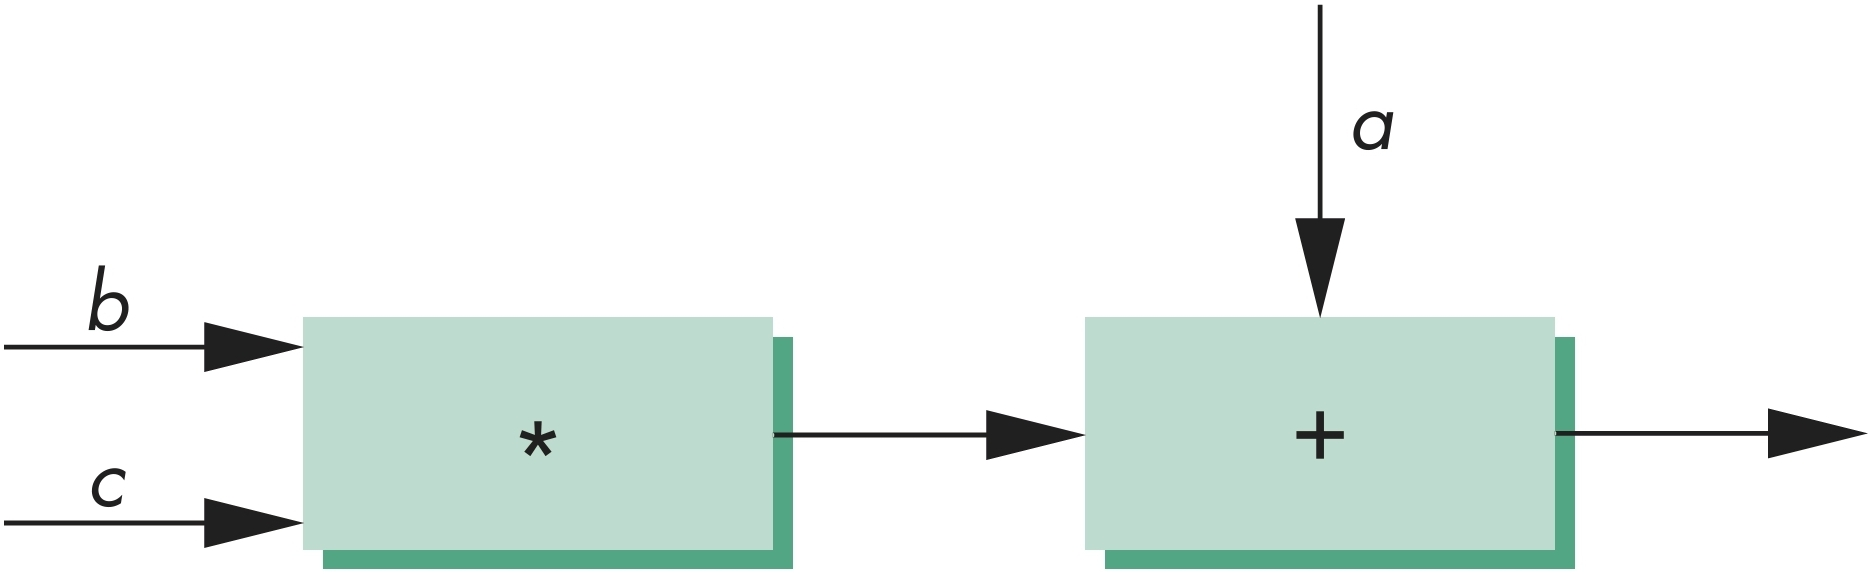
\includegraphics[width=0.48\textwidth]{\main/images/chapter01/arithmetic_pipeline.png}
						\end{center}
						\caption{Arithmetic Pipeline}
					\end{wrapfigure}
					In this pipeline, there is an adder and a multiplier.
					If we use this configuration to computer $a + (b * c)$,
					the calculation takes one multiplication and one addition
					-- the same amount of work required if we use a single processor
					to carry out both operations.

					However, suppose that we have to carry out the same computation
					with many values of $a$, $b$, and $c$.
					Now, the multiplier can pass on the results of its calculation
					to the adder,
					and can start its next multiplication
					while the adder carries out the second step of the calculation
					on the first set of data.

					Whereas it takes the same amount of time to calculate the results
					for any one set of data,
					when working on two sets of data at one time,
					the total time for calculation is shortened markedly.
					In this pipeline, the \concept{throughput} of the system
					has been doubled.
				\end{example}

				\begin{definition}{Throughput}
					The rate at which data flow through the system.
				\end{definition}

				As we add more boxes to a pipeline,
				it takes more time for a single datum to pass through the system.
				This time is called the \concept{latency} of the system.
				The latency must be balanced against the increased throughput
				when evaluating the performance of a system.

			\subsection{The Graphics Pipeline}
				Start with a set of objects.
				Each object comprises a set of graphical primitives.
				Each primitive comprises a set of vertices.
				The collection of primitive types and vertices define
				the \concept{geometry} of the scene.
				The vertices that define the objects
				must be processed similarly to form an image in the framebuffer.

				\begin{sidenote}{Four Major Steps in the Imaging Process}
					\begin{enumerate}
						\item Vertex processing
						\item Clipping and primitive assembly
						\item Rasterization
						\item Fragment processing
					\end{enumerate}

					\begin{center}
						
\includegraphics[width=0.9\textwidth]{\main/images/chapter01/graphics_pipeline.png}
						\captionof{figure}{Geometric Pipeline}
					\end{center}
				\end{sidenote}

			\subsection{Vertex Processing}
				Each vertex is processed independently.
				The major function of this block is to carry out coordinate transformations.
				It can also compute a color for each vertex
				and change any other attributes of the vertex.

				Many of the steps in the imaging process
				can be viewed as transformations between representations of objects
				in different coordinate systems.
				The internal representation of objects
				-- whether in the camera coordinate system or a system used by the graphics software
				-- must eventually be represented in terms of the coordinate system of the display.

				We can represent each change of coordinate systems by a matrix.
				We can represent successive changes in coordinate systems by
				multiplying, or \concept{concatenating}, the individual matrices
				into a single matrix.
				Because multiplying one matrix by another matrix yields a third matrix,
				a sequence of transformations is a candidate for a pipeline architecture.
				The matrices used in computer graphics are small ($4 \times 4$),
				so parallelism can be used within the transformation blocks in the pipeline.

				After multiple stages of transformation,
				the geometry is transformed by a projection transformation.
				In general, we want to keep three-dimensional information as long as possible,
				as objects pass through the pipeline.

				The assignment of vertex colors can be
				as simple as the program specifying a color,
				or as complex as the computation of a color
				from a physically realistic lighting model that
				incorporates the surface properties of the object and
				the characteristic light sources in the scene.

			\pagebreak

			\subsection{Clipping and Primitive Assembly}
				We must do clipping because of the limitation that
				no imaging system can see the whole world at once.
				The human retina has a limited size corresponding to
				an approximately 90-degree field of view.
				Cameras' fields of view can be adjusted by selecting different lenses.

				We obtain the equivalent property in the synthetic camera by considering
				a \concept{clipping volume}.
				The projections of objects within this volume appear in the image.
				Those that are outside do not,
				and are said to be clipped out.
				Objects that straddle the edges of the clipping volume are
				partly visible in the image.

				Clipping must be done on a primitive-by-primitive basis
				rather than on a vertex-by-vertex basis.
				Thus, within this stage of the pipeline,
				we must assemble sets of vertices into primitives,
				before clipping can take place.
				Consequently, the output of this stage is a set of primitives
				whose projections can appear in the image.

			\subsection{Rasterization}
				The primitives that emerge from the clipper are still
				represented in terms of their vertices
				and must be converted to pixels in the framebuffer.

				The output of the rasterizer is a set of \concept{fragments}
				for each primitive.

				\begin{definition}{Fragment}
					Can be thought of as a potential pixel
					that carries with it information,
					including its color and location,
					that is used to update the corresponding pixel in the framebuffer.

					Fragments can also carry along depth information
					that allows later stages to determine whether a particular fragment
					lies behind other previously rasterized fragments for a given pixel.
				\end{definition}

			\subsection{Fragment Processing}
				This stage takes in the fragments generated by the rasterizer
				and updates the pixels in the framebuffer.
				If the application generated three-dimensional data,
				some fragments may not be visible
				because the surfaces they define are behind other surfaces.

				The color of a fragment may be altered by texture mapping or bump mapping.
				The color of the pixel that corresponds to a fragment
				can also be read from the framebuffer
				and blended with the fragment's color
				to create translucent effects.

		\pagebreak

		\section{Programmable Pipelines}
			None of the other approaches to graphics
			can achieve real-time behavior,
			that is, the ability to render complex dynamic scenes
			so that the viewer sees the display without defects,
			in the way pipelining can.
			The commodity graphics market is dominated by graphics cards
			that have pipelines built into the graphics processing unit.

			For many years, these pipeline architectures had a fixed functionality.
			While the application program could set many parameters,
			the basic operations available within the pipeline were fixed.

			Now, both the vertex processor and the fragment processor are
			programmable by the application programmer.
			This means that many of the effects that could not be done in real time,
			as they were not part of the fixed-function pipeline,
			can now be done in real-time.
			An example of this is bump mapping.

			\concept{Vertex shaders} can alter the location or color of each vertex
			as it flows through the pipeline.
			Thus, we can implement a variety of light-material models
			or create new kinds of projections.
			\concept{Fragment shaders} allow us to use textures in new ways
			and to implement other parts of the pipeline,
			such as lighting,
			on a per-fragment basis rather than per-vertex.

			The speed and parallelism in programmable GPUs
			make them suitable for carrying out high-performance computing
			that does not involve graphics.

\end{document}